\section{System Calls}

	\defn{System Call}{the software, typically written in a high-level language (e.g C), which sits between the hardware and the applications}

	\defn{User mode}{restricted level where most programs run without direct access to memory or hardware}

	\defn{Kernel mode}{unrestricted program execution}

	\par{Programs running on user mode are provided an API by the OS which provides the application which mediated access to the hardware. A classical example is a basic task like writing to and reading from a file.}

	\subsection{Parameter Passing}

		\par{In order to pass parameters to the system call we can:}

		\begin{itemize}
			\item use registers
			\item stored them in memory and address of the block passed in register
			\item push onto the stack by the program and pop by OS
		\end{itemize}

	\begin{figure}[H]
		\begin{center}
		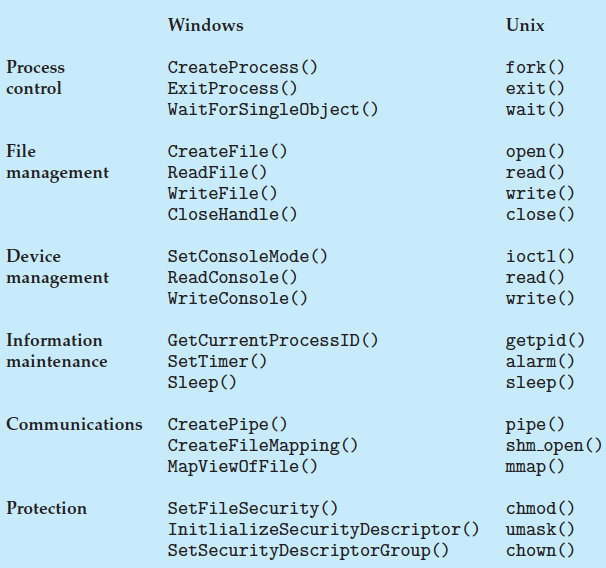
\includegraphics[width=\textwidth]{syscalls}
		\end{center}
	\end{figure}

\subsection{Program Execution}

	\par{As we've seen above the difference between a program and process is that a process is a program being executed. Note than that one program can spawn several processes, i.e for the same file on disk (the written code) multiple requests to resources might happen (e.g multiple tabs on a browser)}

	\subsubsection{Process States}

	\defn{Ready Queue}{an array of active processes waiting to be run}

		\par{Once execution of a program starts a request to the OS is made and the process is added to the \ita{ready queue}. It will then be transitioned into the running state, it can then exit and terminate or can be put into waiting state and back into the ready queue until resources are available for it to finish execution.}

	\begin{figure}[H]
		\begin{center}
		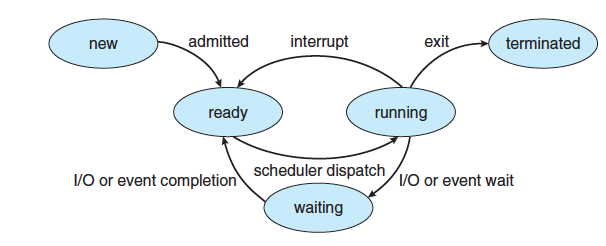
\includegraphics[width=\textwidth]{processState}
		\end{center}
	\end{figure}

	\defn{PCB}{is a data structure used by the OS to store all the information associated with a process}

		\par{For every process the OS keeps a PCB containing all information associated with it, such as state, numbers, counter etc.}

\subsection{Process Creation}

\defn{Process Tree}{a hierarchical representation of processes}

\defn{Boot Loader}{is the program stored in the ROM responsible for loading data and programs into RAM}

\defn{Zombie Process}{a child process which is not \ita{reaped} by its parent upon termination, hence it still exists in the process table}

\defn{Orphan Process}{a child process which is inherited by \texttt{init} because it is still running despite its parent having terminated}

	\par{Processes are spawned by other processes, creating what is know as a \ita{process tree}. When a machine starts there is a single process , the \ita{boot loader} which is responsible for loading the OS into the main memory, this is usually done in multiple stages where simpler programs load increasingly more complex ones, a process know as \ita{chain loading}.}
	\par{The system calls responsible for the creation of processes are:}

		\begin{itemize}
			\item[] \texttt{fork(2)} - takes a process and creates a copy of it
			\item[] \texttt{exec(3)} - family of functions which takes one of the processes and replaces its code with another program's code
			\item[] \texttt{wait(2)} - stops the running process and waits for one of its children to terminate
		\end{itemize}

	\par{By default parent and children processes run concurrently, and the parent waits for the children to terminate. There are multiple level of resource sharing, between sharing all to none.}

	\rem{It could happen that a parent process may fail to \ita{reap} its children state after execution, in which case a \ita{zombie} process is created, which keeps using resources in the background. If the opposite happens, i.e if the parent finishes first then the child process becomes \ita{orphan}}

	\begin{figure}[H]
		\begin{center}
		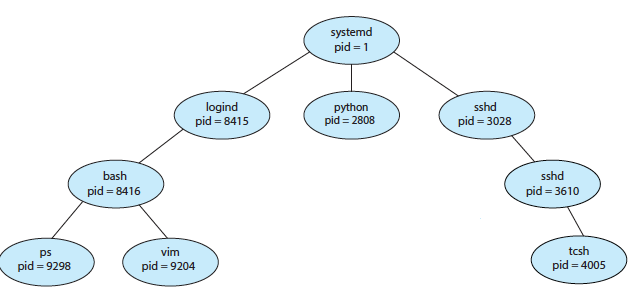
\includegraphics[width=\textwidth]{processTree}
		\end{center}
	\end{figure}


\section{Inter-Process Communication}

	\par{Processes can be independent running in isolation or cooperative sharing data. Cooperating processes can be affected by other processes, which can lead to a chain failure. However, cooperating processes can often be more efficient, since they share information, are more modular and more convenient to run.}

	\subsection{Communication Models}

		\par{It follows that if two processes are cooperating then they need to be able to communicate with each other. There are two possible modes of communication, \ita{message passing} and \ita{shared memory}. In the former processes communicate by sending calls to each other via a message queue in the latter a space of shared memory is allocated where  both processes can read and write.}
		\par{Both processes are often implemented within the same system. The shared memory model is particularly useful when large amounts of data need to be shared; it is also faster since it only uses system calls to establish the region in memory. The message passing model on the other hand is easier to implement in distributed systems, hence it is usually applied when small amounts of data need to be shared.}


	\subsubsection{Message Passing}

		\par{A message passing model has to provide at least two operations \texttt{send} , \texttt{receive}. There are however several factors to consider when implementing these:}

		\begin{itemize}
			\item Directly : If the communication is implemented \ita{directly}, then processes much name each other, if both the receiver and sender are named then the communication is said to be \ita{symmetric}. On the other hand, if only the recipient is explicitly named then one calls it \ita{asymmetric}. 
			\item Indirectly : If the communication is implemented \ita{indirectly} the messages are sent and received via \ita{mailboxes}. Unlike before, links are not necessarily $1-1$ since many processes can share a mailbox. Once a mailbox is created by an initial process, other processes access to the mailbox can be mediated via system calls.
			\item Synchronization : if when performing a \texttt{send, receive} the actor is blocked, then we say that the process is \ita{synchronous}, if the opposite is true then it is \ita{asynchronous}
			\item Buffering : The size of the queue can be either 0, in which case sender must wait for receiver; may be bounded by $n$, in which case the sender must wait if queue is full , or may be unbounded where the sender can keep adding to the queue without restrictions.
		\end{itemize}

	\subsubsection{Shared Memory}

		\rem{See future lecture on memory management}

